
\documentclass[border=12pt]{article} 
\usepackage[dvipsnames]{xcolor}
\usepackage{tikz}
\usepackage[lining]{libertine}
\usepackage[]{xcolor}
\newenvironment{tightcenter}{%
  \setlength\topsep{-20pt}
  \setlength\parskip{-10pt}
  \begin{center}
}{%
  \end{center}
}

\usetikzlibrary{shadows}
\begin{document}
\LARGE
  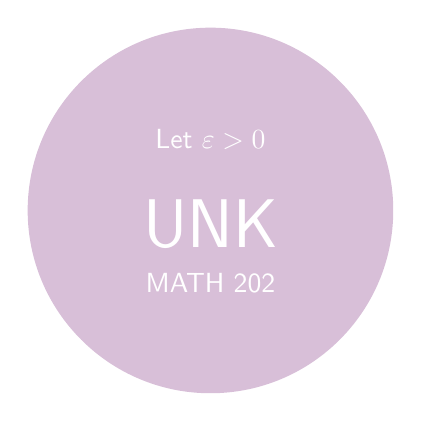
\begin{tikzpicture}
    \node[circle,minimum width=1.5in,text=white,fill=Thistle,font=\sffamily] at (0,0) {  \begin{minipage}[c]{1.5in}  
        \begin{tightcenter}  
            Let \(\varepsilon  > 0 \)  \end{tightcenter}  \hfill  \\ 
             \begin{tightcenter}  \Huge UNK   
 \end {tightcenter} \hfill   \\   
 \begin{tightcenter} MATH 202   \end{tightcenter} \end{minipage} };
  \end{tikzpicture}


\end{document}
